\documentclass[notitlepage]{article}
%\usepackage{lmodern}
%\usepackage[T1]{fontenc}
%\usepackage[spanish]{babel}	
\usepackage[utf8]{inputenc}
\usepackage{amsmath}
\usepackage{amsfonts}
\usepackage{amssymb}
\usepackage{amsthm}
\usepackage{hyperref}
\usepackage{graphicx}
\author{David Cardozo}
\title{Textbook notes on Abstract Algebra}

\newtheorem{thm}{Theorem}
\newtheorem{lem}[thm]{Lemma}
\newtheorem{prop}{Proposition}[section]

\theoremstyle{definition}
\newtheorem{define}{Definition}[section]
\newtheorem{defn}{Definition}[section]
\newtheorem{conj}{Conjecture}[section]
\newtheorem{exm}{Example}[section]
\theoremstyle{remark}
\newtheorem*{rem}{Remark}
\newtheorem*{note}{Note}
\newtheorem{case}{Case}
\newtheorem{exc}{Exercise}
\newtheorem*{sol}{Solution}

\newcommand{\normal}{\triangleleft}


\begin{document}
	
Last class notes:

\textbf{Sylow:} \[ \left| G \right| = p^{\alpha}m, p \not| m \]
we have $ \varnothing \neq \operatorname{Syl}_p(G) \ni P $
\[ 0 < n_p = \left| \operatorname{Syl}_p(G) \right| | m \]
\[ n_p = 1 +kp = \left[ G : N_G(P) \right] \]

Now consider: $ \left| G \right| = p^2 q $, $ p,q $ are distinct primes.
Looking for nomal sylow subgroups. $ P \in \operatorname{Syl}_P, Q \in \operatorname{Syl}_q $
\begin{itemize}
	\item \[ p < q \implies \begin{cases}
	n_q = 1 \implies Q \normal G \\
	n_q > 1 \implies n_q = 1 + tq | p^2 \implies 1 < 1 +tq | p^2
	\end{cases} \]
\end{itemize}

From the second \[ \implies \begin{cases}
 1 +tq = p \textrm{ not posible } \\
 1+tq = p^2 \implies q | p^2 -1 = (p-1)(p+1) \implies 
 \begin{cases}
 q | p -1 \implies \textrm{ not posible } \\
 q| p+1 \implies q = p +1 \implies p = 2, q =3 \rightarrow \left| G \right| = 12
 \end{cases}
\end{cases} \]

Now consider 
$  \left|G\right| = 12 $ Either $ G $ has a normal sylow 3-subgroup or $ G \cong A_4 $.
\[ 1 < n_3 = 1 + 3k | 4 \implies n_3 = 4 \]
so that:
\[ \operatorname{Syl}_3(G) = \left\lbrace P = P_1, P_2,P_3, P_4 \right\rbrace \]
\[ P_i \cap P_j = \left\lbrace 1 \right\rbrace \textrm{ if } i \neq j \]
$ G $ has $ 8 $ elements of order $ 3 $.
\[ \left[ G : N_G(P) \right] = n_3 = 4 \implies N_G(P) = P \]
\[ = \left[G:P\right] \]
Now act by conjugation:
\[ \phi: G \xrightarrow{Conjugation} S_4 \]
we can show that the above map is an injection. (Prove it)
\[ K = \operatorname{Ker}{\phi} \leq N_G(P) = P \]
$ P $ is not normal
Conjugation on \[ \operatorname{Syl}_3 (G) \implies K = 1 \]

Now by 1st isomorphism theorem:
\[ G \cong \phi(G) \leq S_4 \implies \phi(G) = A_4 \]


\begin{figure}[h!]
\centering
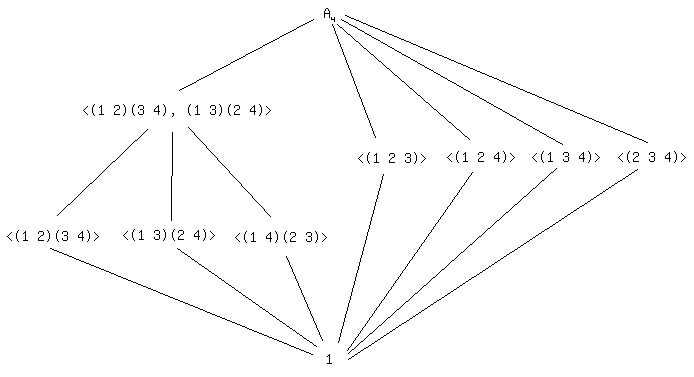
\includegraphics[width=0.8\linewidth]{SubgroupA4}
\caption{}
\label{fig:SubgroupA4}
\end{figure}





We identify: Sylow 2-subgroup $ < (12)(34),(13)(24) > $, and $ <(123)> <(124)> <(134)> $

We observer that normal Sylow 2-subgroup $ A_4 $ has $ 8 $ elements of order $ 3 $-Complement


About the exam:
\begin{itemize}
	\item Class equation: very likely
	\item Semi-direct Product (Favorite)
	\item Automorphisms of $ D_8 $
	\item Inductive argument ascending and descending chain (pag. 195 )
	\item Lot of Sylow Stuff
	\item Iso for Rings
	\item Read the examples for Ring sections.
	\item One very difficult question
	
\end{itemize}




\end{document}